%
%
%\begin{itemize}
%	\item performance of a packet-switching fabric using the NoC -- different topologies, includes interface
%\end{itemize}
%
%

%\subsubsection{Design}

%Packet switching applications switch data that has been separated into packets. 
%These packets include control information that describe various attributes of the payload, such as its source and destination. 
%Unlike other data streaming applications, the distribution of packet sources and destinations can vary widely, and are rarely known before runtime. 
%A Ethernet switch must be capable of completing packet transmission under any possible traffic condition.

\begin{figure*}[t] \centering \vspace{0cm}
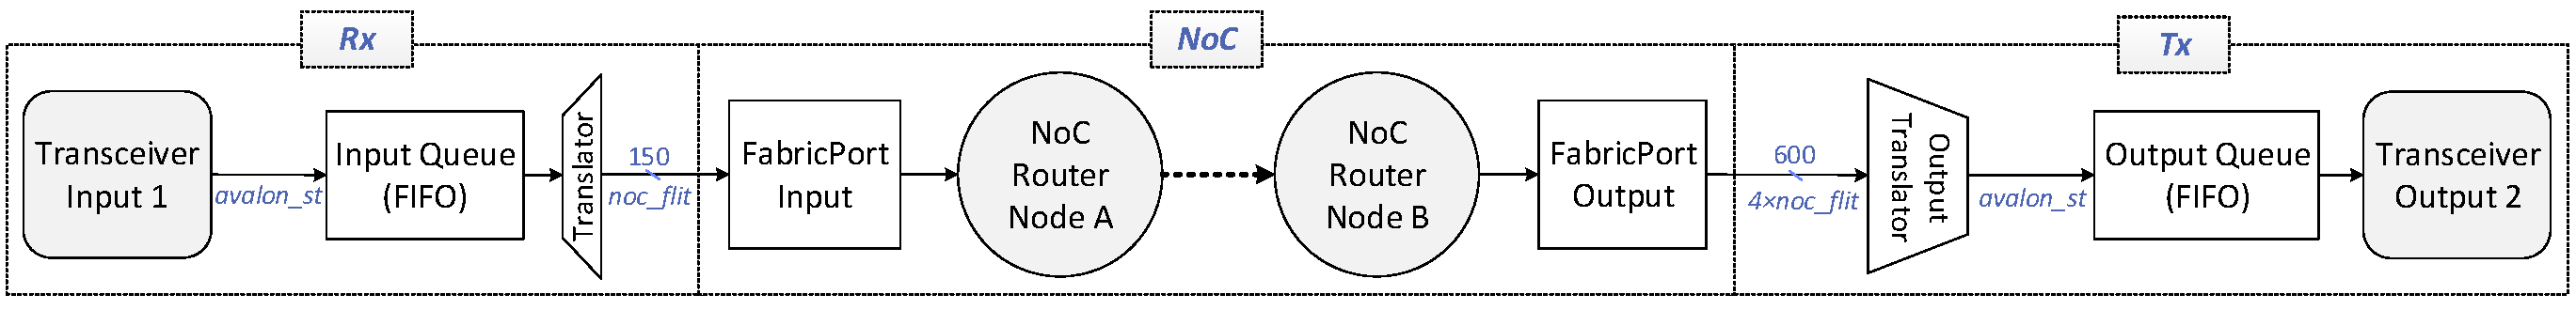
\includegraphics[width=0.95\textwidth, trim = 0cm 0.15cm 0cm 0.3cm]{images/complete-switch-path-new.pdf}
\caption{Functional block diagram of one path through our NoC Ethernet switch.}
\label{fig:switch-blk-diagram}
\vspace{0cm}
\end{figure*}

One of the most important and prevalent building blocks of communication networks is the Ethernet switch.
The embedded NoC provides a natural back-bone for an Ethernet switch design, as it includes (1) switching and (2) buffering within the NoC routers, and (3) a built-in backpressure mechanism for flow control.
Recent work has revealed that an Ethernet switch achieves significant area and performance improvements when it leverages an NoC-enhanced FPGA~\cite{Bitar2014}.
We describe here how such an Ethernet switch can take full advantage of the embedded NoC, while demonstrating that it considerably outperforms the best previously proposed FPGA switch fabric design~\cite{dai-zhu}.

\newpage

%The NoC provides two possible design options for transporting packetized data, as listed below. 
%We will refer to the streaming data packets as ``stream packets'' in order to avoid confusion with the NoC's packets.
%
%\begin{enumerate}
%
%\item \textbf{Encapsulate} each stream packet into multiple NoC packets. 
%A NoC packet holds one data beat from the stream packet, including both payload and all control information. 
%The stream packet's control data does not need to be read.
%
%\item \textbf{Translate} each stream packet into a single NoC packet. 
%The stream packet's start-of-packet (SOP) and end-of-packet (EOP) data beats are sent in the head and tail flits of the NoC packet, respectively. 
%Thus, the SOP and EOP signals are stripped from the stream packet before being sent through the NoC. 
%
%\end{enumerate}
%
%Encapsulating the data is the simplest design option, as it only requires logic to read the data's destination before sending it through the NoC.
%Additionally, since it breaks up stream packets into smaller, fixed-size NoC packets, it can potentially achieve better latency.
%However, this design method comes with several limitations.
%Breaking packets up into smaller units introduces the possibility of packet re-ordering and packet interleaving in the NoC.
%%A centralized scheduler, similar to ones used in other Ethernet switch designs, would be needed to prevent this from occurring.
%To remedy this, each NoC packet would need additional control data indicating the flit ID and source, as well as complex re-ordering logic at the output.
%On the other hand, translating each stream packet to a NoC packet prevents packet re-ordering/interleaving, thus removing this complexity.
%Although translation requires some additional logic to perform the conversion from stream packet to NoC packet, and vice versa, this logic is far simpler than the re-ordering logic necessary for encapsulation.
%Thus, we recommend that Ethernet switch designs translate, rather than encapsulate, stream packets into NoC packets.
%%By building and simulating this design, we show that it better leverages the NoC for packet-switching applications.

%\begin{figure}[t] \centering \vspace{0cm}
%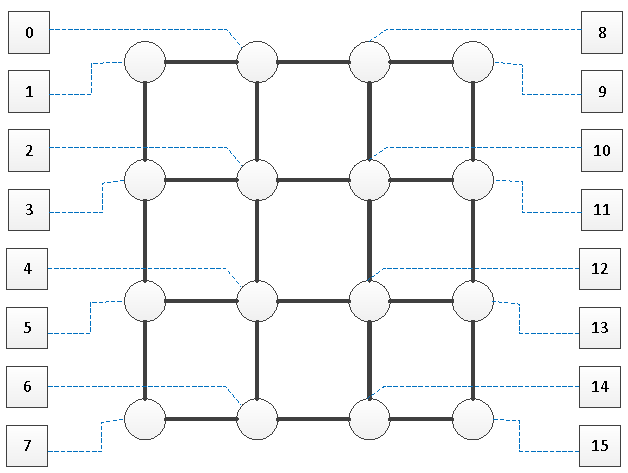
\includegraphics[width=0.4\textwidth]{images/16-node-mesh.pdf}
%\caption{Each of the 16 transceiver nodes (squares) connect to a unique NoC router (circles) through the FPGA's fabric (dashed lines)}
%\label{fig:16mesh}
%\vspace{0cm}
%\end{figure}

%Our design consists of a 16$\times$16 10-Gigabit Ethernet switch.
The embedded NoC is used in place of the switch's crossbar.
For a 16$\times$16 switch, each of the 16 transceiver nodes are connected to one of the 16 NoC routers via the FPGA's soft fabric.
%To transport 10~Gb/s data, the soft fabric is set to run at 156.25 MHz for 64-bit wide data.
%Each transceiver-to-router path consists of buffering and logic to convert stream packets to NoC packets, and vice-versa.
%The transceiver-to-router paths complete the flow shown in Fig.~\ref{fig:switch-blk-diagram}.
Fig.~\ref{fig:switch-blk-diagram} shows the path between transceiver 1 and transceiver 2; in our 16$\times$16 switch there are 256 such paths from each input to each output. 
%On the receive path (\textit{Rx}), two stream flits (\textit{avalon\textunderscore st}) are joined together (\textit{2$\times$avalon\textunderscore st}) before being inserted into an input queue.
On the receive path (\textit{Rx}), Ethernet data is packed into NoC flits before being brought to the FabricPort input.
The translator sets NoC control bits such that one NoC packet corresponds to one Ethernet frame.
For example, a 512-byte Ethernet frame is converted into 32 NoC flits.
%If the NoC router's input fabric port is ready to accept data, the input queue ejects flits to the translator, which adds the necessary NoC control bits and strips the unnecessary Avalon Stream control bits (valid, SOP, EOP) before injecting the newly-created NoC flit into the fabric port.
After the NoC receives the flit from the FabricPort, it steers the flit to its destination, using dimension-order XY routing.
%\footnote{The impact of routing algorithms on NoC-based Ethernet switch performance was investigated by Bitar \textit{et al.}~\cite{Bitar2014}.}
%On the transmit path (\textit{Tx}), round-robin arbitration logic is needed, as the FabricPort can output up to four NoC flits from the same packet in the same cycle (see Section~\ref{sec_fabricport}).
%On the transmit path (\textit{Tx}), the translator uses demultiplexing in order to convert the FabricPort output width (600~bits) to the output queue width (150~bits).
On the transmit path (\textit{Tx}), the NoC can output up to four flits (600~bits) from a packet in a single system clock cycle -- this is demultiplexed in the output translator to the output queue width (150~bits).
This demultiplexing accounts for most of the translators area in Table~\ref{tbl:hcost}.
The translator also strips away the NoC control bits before inserting the Ethernet data into the output queue.
%The output queue waits for an end-of-packet signal before beginning transmission.
%Although we set the queue size to be 64 bits wide and 512 words deep, this can be varied depending on the needs of the switch's particular application.
The design is synthesized on a Stratix V device.
A breakdown of its FPGA resource utilization is shown in Table~\ref{tbl:hcost}.
Because we take advantage of the NoC's switching and buffering our switch is \til3$\times$ more area efficient than previous FPGA Ethernet switches~\cite{dai-zhu}.

%The buffering mechanism used by our switch is considered combined input/output queued (CIOQ).
%However, our Ethernet switch has important differences from previously proposed CIOQ architectures~\cite{minkenberg2000combined}.
%The NoC already provides built-in flow control for handling data being sent from multiple sources to a single destination.
%Thus, no centralized scheduling logic or additional flow control signals between the inputs and outputs are necessary, resulting in significant complexity savings.
%%This would not have been possible if the design had encapsulated rather than translated the data, as centralized scheduling logic would have been necessary to 
%Additionally, the NoC mitigates head-of-line blocking (HOL) by buffering packets within the NoC rather than within the input queues.
%Typically, CIOQ architectures use virtual output queues (VOQ) to mitigate HOL~\cite{minkenberg2000combined}, thus revealing additional hardware cost savings for our NoC-based Ethernet switch design.

% --> Only talk about the replacement of scheduling logic by NoC backpressuring. Leave HoL discussion to journal paper?

%\begin{itemize}
%
%\item \textbf{No scheduling logic.} In nearly all Ethernet switch designs, scheduling logic is necessary to control which inputs are granted access to the switch crossbar.
%
%\item \textbf{No head-of-line blocking (HOL).} 
%
%\end{itemize}

% introduce concept of translating data packets to NoC packets along with both options
% describe design (with block diagram) for 16x16 10~Gb/s
% illustrate inherent benefits of this switch: no centralized scheduler needed, no VOQs needed for HOL

%\subsubsection{Evaluation}

Two important performance metrics for Ethernet switch design are bandwidth and latency~\cite{elhanany2005network}.
The bandwidth of our NoC-based Ethernet switch is limited by the supported bandwidth of the embedded NoC.
As described in Section~\ref{sec:hnoc}, the NoC's links have a bandwidth capacity of 22.5 GB/s (180~Gb/s).
Since some of this bandwidth is used to transport packet control information, the NoC's links can support up to 153.6~Gb/s of Ethernet data.
%The worst case traffic pattern that the NoC-crossbar must support is the pattern that places the highest demand on a NoC link while driving the NoC's sinks at no higher than the line rate, $R$ ($R = 10$~Gb/s in our design).
%Analysis of the 16-node mesh reveals that the maximum NoC channel load is $3R$.
%Thus, the maximum supported bandwidth per node for our Ethernet switch is $R = 51.2$~Gb/s, or an aggregate bandwidth of 819.2~Gb/s.
Analysis of the worst case traffic in a 16-node mesh shows that the NoC can support a line rate of one third its link capacity, i.e. 51.2~Gb/s~\cite{Bitar2014}.
While previous work on FPGA switch design has achieved up to 160~Gb/s of aggregate bandwidth~\cite{dai-zhu}, our switch design can achieve 51.2$\times$16 = 819.2~Gb/s by leveraging the embedded NoC.
We have therefore implemented a programmable Ethernet switch with 16 inputs/outputs that is capable of either 10~Gb/s, 25~Gb/s or 40~Gb/s -- three widely used Ethernet standards.

%
%
\begin{table}[!t]
\centering
\begin{small}
    \caption{Hardware cost breakdown of an NoC-based 10-Gb Ethernet switch on a Stratix V device.}
    \label{tbl:hcost}
    \begin{tabular}{ccccccc}
    \toprule
     & 10GbE & I/O & Translators & \textbf{Total} \\
     & MACs & Queues &  & & \\
    \midrule
	ALMs & 24000  & 3707 &  3504 & \textbf{31211} \\ 
	%ALUTs & 32016 & 5616 & 2352 & \textbf{41648} \\
	%Regs  & 49232 & 3264 & 17840 & \textbf{53696} \\
	M20Ks & 0    & 192   & 0 & \textbf{192}   \\
    \bottomrule
    \end{tabular}
\end{small}
\end{table}
%
%

\begin{figure}[t] \centering \vspace{0cm}
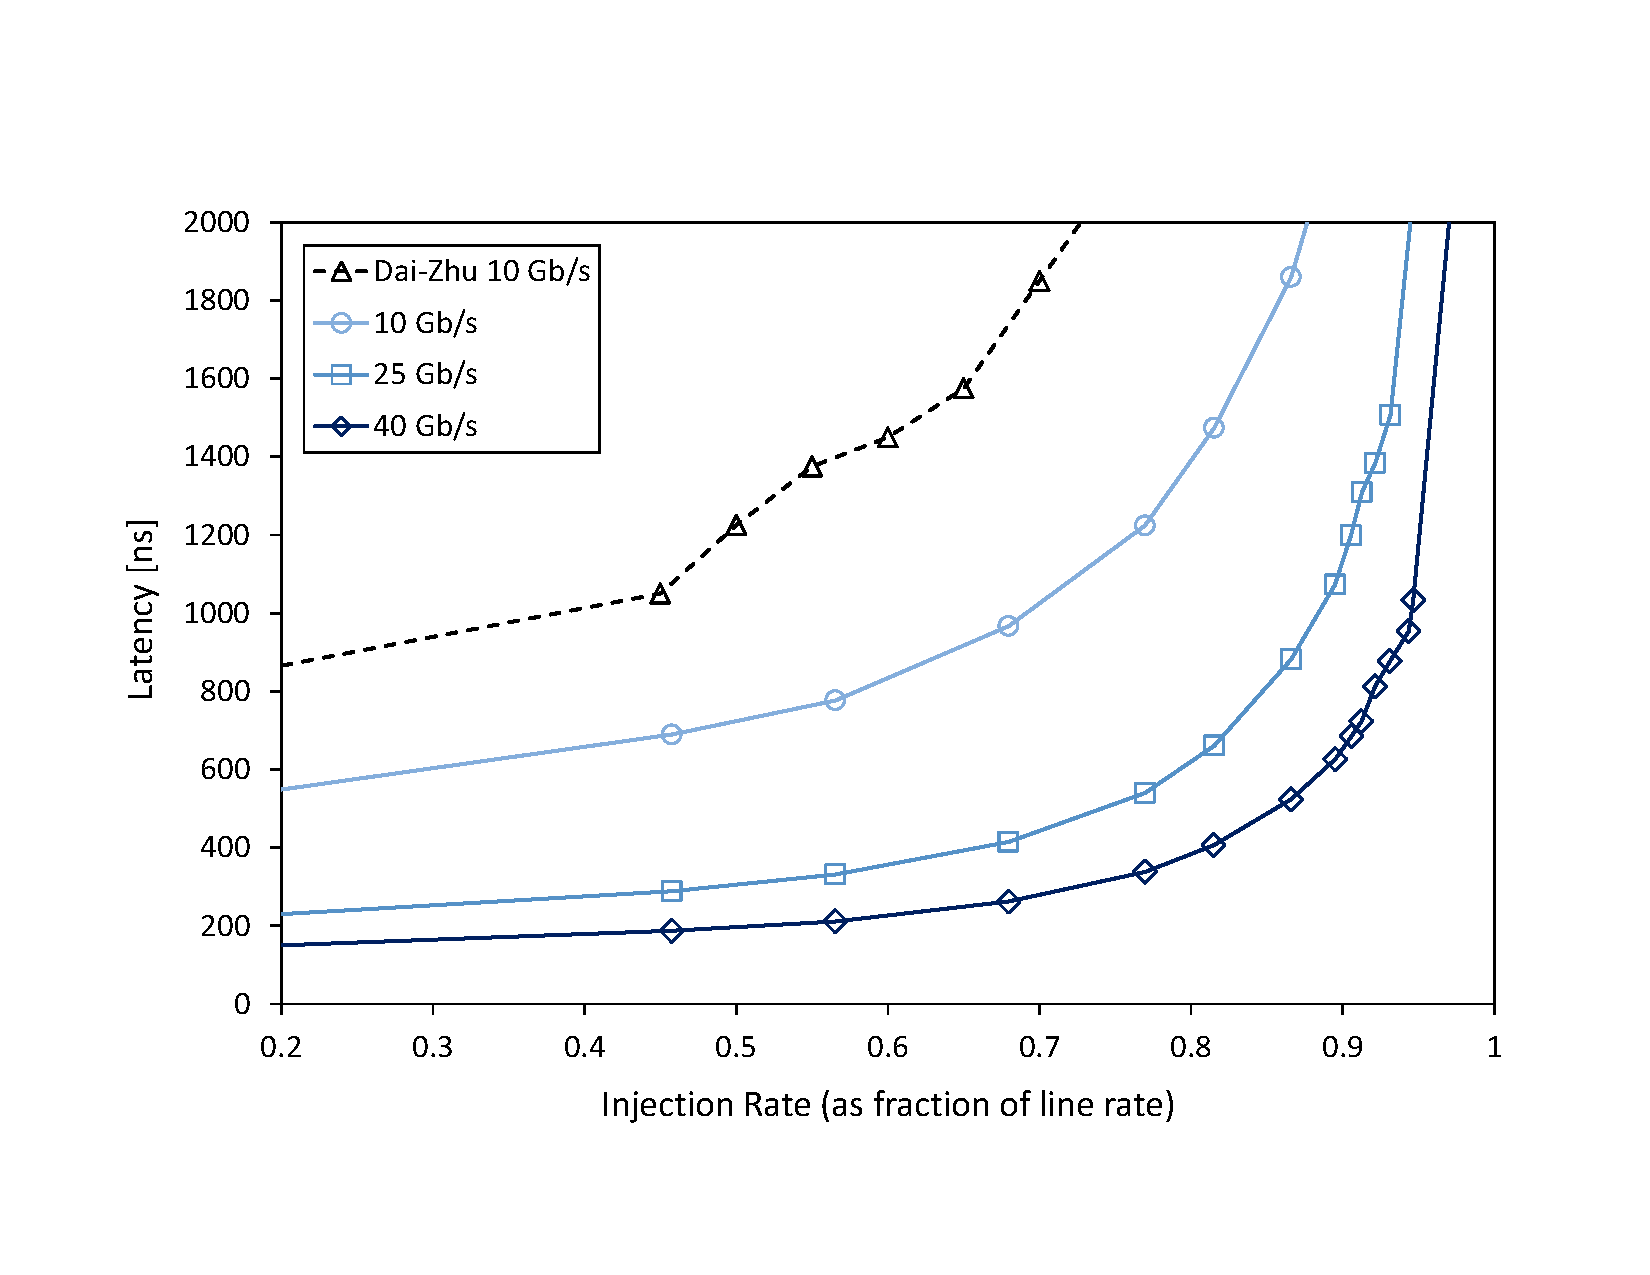
\includegraphics[width=0.485\textwidth, trim = 2cm 2.5cm 2cm 3.4cm, clip]{images/latency-chart-data-320-640.pdf}
\caption{Latency vs. injection rate of the NoC-based Ethernet switch design given line rates of 10, 25, and 40~Gb/s, and compared to the Dai/Zhu 16$\times$16 10~Gb/s FPGA switch fabric design~\cite{dai-zhu}. Our switch queues and Dai/Zhu's switch queues are of size 60kb and 16kb, respectively.}
\label{fig:lat-plot}
\vspace{0cm}
\end{figure}

The average latency of our Ethernet switch design is measured using the \texttt{RTL2Booksim} simulator.
An ON/OFF injection process is used to model bursty, uniform random traffic, with a fixed Ethernet frame size of 512 bytes (as was used in~\cite{dai-zhu}).
Latency is measured as the time between a packet head being injected into the input queue and it arriving out of the output queue.
%The design is simulated at 10, 25, and 40~Gb/s to model modern Ethernet bandwidths, with latency measured and plotted in Fig.~\ref{fig:lat-plot}.
Fig.~\ref{fig:lat-plot} plots the latency of our Ethernet switch at its supported line rates of 10~Gb/s, 25~Gb/s and 40~Gb/s.
Surprisingly, the latency of a 512~byte packet improves at higher line rates.
This is because a higher line rate means a faster rate of injecting NoC flits, and the NoC can handle the extra switching without a large latency penalty thus resulting in an improved overall latency.
%Because the latency of the NoC varies little when the injection bandwidth is below its capacity, NoC-based Ethernet switches of higher throughput inject packets into the NoC at a faster rate and therefore achieve better latency.
No matter what the injection bandwidth, the NoC-based switch considerably outperforms the Dai/Zhu switch~\cite{dai-zhu} for all injection rates.
%The saturation point can be improved by increasing the size of the output queues.
%However, higher throughputs cause the NoC to reach its saturation point at a lower injection rate than lower throughputs.
By supporting these high line rates, our results show that an embedded NoC can push FPGAs into new communication network markets that are currently dominated by ASICs.

%want to say something about programmability being important in these markets, hence the cavium switch.

%Fig.~\ref{fig:lat-plot} plots the latency for both queue depths as a function of the injection rate.
%The ``knee'' in each plot indicates the injection rate at which the output queues become full and start backpressuring the NoC.
%An output queue fills up when it is being driven by multiple sources at the same time, as it can only eject flits at up to the line rate.
%Up until the plot knee, the average latency remains below 65 RTL cycles (156.25 MHz), or 416 ns.

\newpage

